\documentclass{article}

% FIXME: https://github.com/google-research/arxiv-latex-cleaner

\usepackage{arxiv}

\usepackage[utf8]{inputenc} % allow utf-8 input
\usepackage[T1]{fontenc}    % use 8-bit T1 fonts
\usepackage{hyperref}       % hyperlinks
\usepackage{url}            % simple URL typesetting
\usepackage{booktabs}       % professional-quality tables
\usepackage{amsfonts}       % blackboard math symbols
\usepackage{nicefrac}       % compact symbols for 1/2, etc.
\usepackage{microtype}      % microtypography
\usepackage{lipsum}		% Can be removed after putting your text content
\usepackage{graphicx}
\usepackage{float}

\title{A template for the \emph{arxiv} style}

%\date{September 9, 1985}	% Here you can change the date presented in the paper title
%\date{} 					% Or removing it

\author{
  Maciej A.~Czyzewski\\
  Institute of Computing Science\\
  Poznan University of Technology\\
  Piotrowo 2, 60-965 Poznan, Poland\\
  \texttt{maciejanthonyczyzewski@gmail.com} \\
  \And
  Kamil~Piechowiak\\
  Institute of Computing Science\\
  Poznan University of Technology\\
  Piotrowo 2, 60-965 Poznan, Poland\\
  \texttt{kamil.cams@gmail.com} \\
}

\begin{document}

%%%%%%%%%%%%%%%%%%%%%%%%%%%%%%%%%%%%%%%%%%%%%%%%%%%%%%%%%%%%%%%%%%%%%%%%%%%%%%%%

\maketitle

\begin{abstract}
	\lipsum[1]
\end{abstract}

\keywords{First keyword \and Second keyword \and More}

%%%%%%%%%%%%%%%%%%%%%%%%%%%%%%%%%%%%%%%%%%%%%%%%%%%%%%%%%%%%%%%%%%%%%%%%%%%%%%%%

omghahahah

\begin{figure}[H]
	\centering
	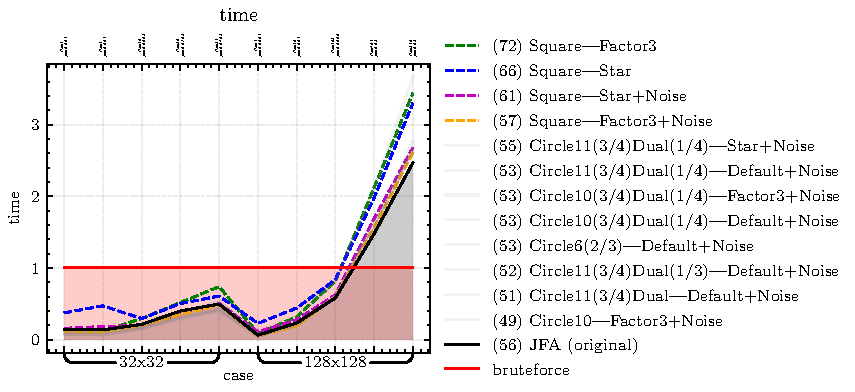
\includegraphics[width=\linewidth]{../figures/figure-1-time}
	\caption{\emph{batchboost} presented in three phases: (a) pairing by sorting
	  error (b) mixing with \emph{mixup} (c) feeding: a mixed feed-batch and new
	  samples in half-batch by 1:1 ratio.}
	\label{fig:abstract}
\end{figure}

\begin{table}
	\centering
	\begin{tabular}{lrrrllr}
\hline
 Algorithm                  &   $\rho$=0.0003 &   $\rho$=0.001 &   $\rho$=0.0099 & $\rho$=0.0298   & $\rho$=0.0499   &   Avg. score \\
\hline
 Square|Factor3             &             0   &           13.2 &            55.5 & \textbf{122.0}  & \textbf{169.3}  &           71 \\
 Square|Star                &             0   &            0   &            41.7 & \textbf{115.2}  & \textbf{161.5}  &           63 \\
 Square|Star+Noise          &            12.3 &           19   &            48.4 & 96.3            & \textbf{142.3}  &           63 \\
 Square|Factor3+Noise       &             7.9 &           13.6 &            43.5 & 91.6            & \textbf{145.2}  &           60 \\
 Circle8Dual|Default        &             0   &            9.8 &            39.3 & 85.6            & \textbf{123.3}  &           51 \\
 Circle10|Star+Noise        &            11.8 &           16.3 &            43.4 & 79.2            & 98.7            &           49 \\
 Circle10Dual|Factor3+Noise &             5.5 &           10.9 &            37.8 & 81.4            & \textbf{110.6}  &           49 \\
 Circle8Dual|Factor3+Noise  &             6.8 &           12.7 &            42.2 & 82.7            & 94.2            &           47 \\
 Circle10Dual|Star          &             0   &            0   &            28.2 & 85.0            & \textbf{124.2}  &           47 \\
 Circle11Dual|Factor3+Noise &             6   &           12   &            35.2 & 76.9            & \textbf{107.2}  &           47 \\
 Circle10Dual|Factor3       &             0   &            4.8 &            40.8 & 80.2            & \textbf{109.3}  &           47 \\
 Circle12|Star+Noise        &            10.6 &           14.7 &            37   & 70.3            & 87.2            &           43 \\
 Circle13|Factor3+Noise     &             6.2 &           10.4 &            32.6 & 70.9            & 92.2            &           42 \\
 Circle15Dual|Star          &             0   &            1.6 &            35.8 & 68.2            & \textbf{101.9}  &           41 \\
 Circle17Dual|Star          &             0   &            1.3 &            34.4 & 65.0            & 95.4            &           39 \\
 Circle6|Factor3+Noise      &             7.7 &           15.7 &            53.2 & 79.6            & 34.9            &           38 \\
 Circle7Dual|Default        &             0   &            6.4 &            37   & 66.7            & 79.7            &           37 \\
 Circle6Dual|Default        &             0   &            4.8 &            36.2 & 67.2            & 79.0            &           37 \\
 Circle6Dual|Star+Noise     &            14.7 &           20.9 &            42.1 & 59.2            & 32.4            &           33 \\
 Circle8Dual|Star           &             0   &            0   &             0   & 49.0            & 78.7            &           25 \\
 Circle9Dual|Star           &             0   &            0   &             0.2 & 39.1            & 74.9            &           22 \\
 Circle9Dual|Factor3        &             0   &            0   &             5.4 & 35.9            & 69.9            &           22 \\
 SquareDual|Factor3         &             0   &            4.9 &            19.2 & 35.8            & 49.8            &           21 \\
 Circle8Dual|Factor3        &             0   &            0   &             5.8 & 37.6            & 64.2            &           21 \\
 Circle10|Factor3           &             0   &            1.1 &            12.9 & 32.5            & 52.6            &           19 \\
 Circle14|Factor3           &             0   &            1   &            10.7 & 36.4            & 50.1            &           19 \\
 Circle9|Factor3            &             0   &            1.1 &             9.5 & 31.6            & 46.0            &           17 \\
 Circle10|Star              &             0   &            0   &             2.8 & 30.9            & 49.0            &           16 \\
 SquareDual|Default+Noise   &             2.1 &            3.5 &            12.3 & 26.7            & 37.8            &           16 \\
 Circle7Dual|Factor3        &             0   &            0   &             0   & 2.5             & 0.0             &            0 \\
 Circle7Dual|Star           &             0   &            0   &             0   & 1.9             & 0.0             &            0 \\
 Circle6Dual|Star           &             0   &            0   &             0   & 0.0             & 0.1             &            0 \\
\hline
\end{tabular}
	\newline
	\caption{domain: 32x32, 64x64, 128x128, 256x256}
\end{table}

%%%%%%%%%%%%%%%%%%%%%%%%%%%%%%%%%%%%%%%%%%%%%%%%%%%%%%%%%%%%%%%%%%%%%%%%%%%%%%%%

\bibliographystyle{unsrt}
\bibliography{references} 

\end{document}
